% ============================================================
%  ASKVISA.IN — Empirical Website Analysis Research Paper
%  Class   : IEEEtran (IEEE Transactions / Journal style)
%  Engine  : pdfLaTeX
%  Author  : Milan Pandavadra
%  Version : 7.0 — Extended Edition (April 2026)
% ============================================================

\documentclass[journal, 10pt, twoside]{IEEEtran}

% ── Core Packages ───────────────────────────────────────────
\usepackage[T1]{fontenc}
\usepackage[utf8]{inputenc}
\usepackage{microtype}
\usepackage{times}

% ── Math & Symbols ──────────────────────────────────────────
\usepackage{amsmath, amssymb, amsfonts}
\usepackage{bm}

% ── Graphics, Figures, TikZ ─────────────────────────────────
\usepackage{graphicx}
\usepackage{float}
\usepackage{subcaption}
\usepackage{tikz}
\usepackage{pgfplots}
\pgfplotsset{compat=1.17}
\usetikzlibrary{shapes.geometric, arrows.meta, positioning,
                fit, backgrounds, calc}

% ── Algorithms ──────────────────────────────────────────────
\usepackage{algorithm}
\usepackage{algpseudocode}

% ── Tables ──────────────────────────────────────────────────
\usepackage{booktabs}
\usepackage{multirow}
\usepackage{tabularx}
\usepackage{array}
\usepackage{longtable}
\usepackage{enumitem}
\usepackage{pifont}
\newcommand{\cmark}{\ding{51}}
\newcommand{\xmark}{\ding{55}}

% ── Colours ─────────────────────────────────────────────────
\usepackage[dvipsnames, table]{xcolor}
\definecolor{askblue}{RGB}{0, 84, 166}
\definecolor{darkgray}{RGB}{100,100,100}
\definecolor{codegreen}{rgb}{0,0.6,0}
\definecolor{codegray}{rgb}{0.5,0.5,0.5}
\definecolor{codepurple}{rgb}{0.58,0,0.82}
\definecolor{backcolour}{rgb}{0.95,0.95,0.92}

% ── Hyperlinks & PDF Metadata ───────────────────────────────
\usepackage[
  colorlinks = true,
  linkcolor  = askblue,
  citecolor  = askblue,
  urlcolor   = askblue,
  pdftitle   = {Ask Visa (askvisa.in): A Functional and UX Analysis of an
                Indian E-Visa Processing Portal},
  pdfauthor  = {Milan Pandavadra},
  pdfsubject = {Web Engineering UX E-Government Travel-Tech},
  pdfkeywords= {E-Visa Travel-Tech Chatbot UX-Analysis India FlyAnyTrip}
]{hyperref}

% ── Code Listings ───────────────────────────────────────────
\usepackage{listings}
\lstset{
  backgroundcolor=\color{backcolour},
  commentstyle=\color{codegreen},
  keywordstyle=\color{magenta},
  numberstyle=\tiny\color{codegray},
  stringstyle=\color{codepurple},
  basicstyle=\ttfamily\footnotesize,
  breakatwhitespace=false,
  breaklines=true,
  captionpos=b,
  keepspaces=true,
  numbers=left,
  numbersep=5pt,
  showspaces=false,
  showstringspaces=false,
  showtabs=false,
  tabsize=2
}

% \IEEEoverridecommandlockouts

% ============================================================
\begin{document}

% ── Title ────────────────────────────────────────────────────
\title{Ask Visa (askvisa.in): A Functional, UX, and Security Analysis
of a Conversational E-Visa Processing Portal for the Indian Market}

\author{%
  \IEEEauthorblockN{Milan Pandavadra\IEEEauthorrefmark{1}}\\
  \IEEEauthorblockA{%
    \IEEEauthorrefmark{1}Department of Computer Science and Engineering,\\
    [Insert College Name], [Insert City, Country]\\
    email: student@university.edu}
}

\maketitle

% ============================================================
%  ABSTRACT
% ============================================================
\begin{abstract}
The digitization of visa processing services in India has accelerated
significantly post-pandemic, producing a new category of consumer-facing
travel-tech platforms that act as intermediaries between applicants and
government immigration authorities. This paper presents a structured
analytical study of Ask Visa (\texttt{askvisa.in}), a live e-visa
processing portal operated by FlyAnyTrip, an Indian travel services
company. The analysis was conducted through direct observation of the
live website, inspection of its application portal, legal documentation,
and public-facing interface components as they exist in April 2026.

Ask Visa supports e-visa processing for five primary destinations ---
Thailand, Dubai (UAE), Singapore, Vietnam, and Malaysia --- with
advertised processing times ranging from two to five days. Its key
architectural features include a ten-step guided application wizard with
a real-time progress indicator, a conversational chatbot assistant with
quick-reply destination buttons, a multi-mode entry point offering new
applications, edits to existing orders, status tracking, and PDF summary
downloads, and a claimed bank-grade secure document upload pipeline.

This paper evaluates the portal across six dimensions: functional
completeness, user experience (UX) design, security and data privacy
posture, compliance with Indian regulatory frameworks, competitive
positioning relative to comparable Indian intermediary platforms, and
mobile and cross-device readiness. We apply Nielsen's usability
heuristics, the Technology Acceptance Model (TAM), and Shneiderman's
Eight Golden Rules as evaluation frameworks, and we examine the
conversion funnel architecture and chatbot design in detail.

We identify specific strengths --- particularly the chatbot-guided
onboarding, the wizard-based form structure, and the WhatsApp support
integration --- and document gaps in trust signalling, post-submission
status transparency, multilingual support, and accessibility compliance.
The study contributes a detailed design audit of a real-world Indian
travel-tech product and proposes a comprehensive, evidence-based roadmap
for portals operating in the visa intermediary category. Broader
implications for the design of high-stakes civic and commercial data
collection interfaces in India's emerging digital economy are also
discussed.
\end{abstract}

\begin{IEEEkeywords}
E-Visa, Travel Technology, Conversational UI, India, FlyAnyTrip,
UX Analysis, Wizard Interface, Web Security, PII, Digital Intermediary.
\end{IEEEkeywords}

% ============================================================
%  1. INTRODUCTION
% ============================================================
\section{Introduction}
\label{sec:introduction}

India is among the largest sources of outbound international travelers
globally. According to the Ministry of Tourism, Government of India,
outbound international departures exceeded 27 million in 2023 and continue
to recover toward the pre-pandemic peak. A significant proportion of these
travelers require e-visas for their destinations --- Thailand, Dubai,
Singapore, Vietnam, and Malaysia consistently rank among the top five
outbound destinations for Indian passport holders.

Obtaining an e-visa through official government channels, while technically
possible for most of these destinations, involves navigating unfamiliar
foreign-language portals, strict document format requirements, and opaque
processing timelines. This friction has created a sizable market for
third-party visa processing services that act as intermediaries: collecting
applicant documents, verifying them, and submitting applications on the
applicant's behalf for a service fee. Dozens of such platforms now operate
in India, ranging from unorganized WhatsApp-based consultants to structured
web applications.

Ask Visa (\texttt{askvisa.in}) represents the more structured end of this
spectrum. It is a purpose-built web portal offering a guided application
workflow, a conversational assistant, document upload, and application
tracking. It is operated under the brand FlyAnyTrip, an Indian company
whose legal entity governs the site's privacy policy and terms of service
under Indian law.

\subsection{Motivation and Research Questions}
\label{subsec:motivation}
While academic literature on e-government portals and visa systems is
growing, very little work critically examines the design and functional
properties of private-sector visa intermediary platforms in the Indian
context. This paper addresses that gap through a direct observational
analysis of \texttt{askvisa.in}. The specific research questions are:

\begin{enumerate}
  \item \textbf{RQ1 --- Functional Coverage:} What functions does Ask Visa
  expose to users, and how completely do they address the end-to-end visa
  application lifecycle?
  \item \textbf{RQ2 --- UX Design Quality:} How well does the interface
  design align with established HCI principles for reducing user cognitive
  load and anxiety in high-stakes interactions?
  \item \textbf{RQ3 --- Security and Privacy Posture:} What data protection
  mechanisms and disclosure practices are implemented, and how do they align
  with applicable Indian law?
  \item \textbf{RQ4 --- Gap Analysis:} What are the most significant
  design and functional deficiencies, and what evidence-based changes
  would address them?
\end{enumerate}

\subsection{Scope and Method}
The analysis was conducted entirely through publicly accessible interfaces
of \texttt{askvisa.in} as observed in April 2026. This includes the landing
page (\texttt{landing.php}), the application portal (\texttt{index.php}),
the Privacy Policy (\texttt{privacy\_policy.php}), and the Terms of Use
(\texttt{terms\_of\_use.php}). No backend systems were probed or tested.
The analysis is strictly observational and evaluative.

\subsection{Paper Organisation}
Section~\ref{sec:background} reviews relevant literature and the Indian
e-visa intermediary market. Section~\ref{sec:siteoverview} provides a
structured overview of the website's observed features.
Section~\ref{sec:ux} evaluates the UX design against established
frameworks. Section~\ref{sec:functional} analyses functional completeness.
Section~\ref{sec:security} examines security and privacy.
Section~\ref{sec:conversion} analyses the conversion funnel and
drop-off risk points. Section~\ref{sec:mobile} assesses mobile and
cross-device readiness. Section~\ref{sec:competitive} positions Ask Visa
against comparable Indian intermediary platforms. Section~\ref{sec:gaps}
identifies gaps and proposes recommendations. Section~\ref{sec:design_patterns}
discusses broader design pattern implications. Section~\ref{sec:discussion}
discusses broader implications. Section~\ref{sec:conclusion} concludes.

% ============================================================
%  2. BACKGROUND AND RELATED WORK
% ============================================================
\section{Background and Related Work}
\label{sec:background}

\subsection{E-Visa Processing in India: Market Context}
India's travel-tech ecosystem has matured rapidly. Platforms such as
MakeMyTrip, Yatra, and EaseMyTrip have dominated the flight and hotel
booking segment. The visa processing sub-segment, however, is less
consolidated, with a fragmented landscape of small consultancies, travel
agencies, and newer purpose-built portals. The COVID-19 pandemic disrupted
outbound travel sharply, but also accelerated digital adoption among
consumers who were previously accustomed to in-person visa consultants.

FlyAnyTrip positions itself as a fully digital alternative: documents are
uploaded through the browser, communication occurs through the platform
and WhatsApp, and the output (the e-visa) is delivered by email. This
model reduces the logistical friction of physically visiting a visa
processing center but introduces new design and trust challenges that
are the subject of this analysis.

\subsection{Conversational UI in Service Applications}
The use of chatbots and conversational interfaces in travel and e-government
applications has grown substantially. Gnewuch et al.\ (2017) found that
conversational agents reduce perceived effort in form-filling tasks by
presenting questions sequentially rather than as a flat list, which aligns
with cognitive load theory. Ask Visa's chatbot assistant, which presents
a welcome message and destination quick-buttons before launching the
application wizard, is an implementation of this principle.

Shum et al.\ (2018) distinguish between task-oriented chatbots (designed
to complete a specific transaction) and open-domain chatbots (designed for
general conversation). Ask Visa's assistant is clearly task-oriented ---
its quick-reply options (Thailand, Dubai, Singapore, Malaysia, Check Status)
are scoped exclusively to the visa application workflow. This is the
appropriate design choice for a transactional service context.

\subsection{Multi-Step Wizard Interfaces}
Wizard interfaces --- sequences of focused steps presented one at a time ---
have been studied extensively in the context of complex form completion.
Seckler et al.\ (2014) found that breaking long forms into labelled steps
with visible progress indicators significantly reduces abandonment rates
compared to single-page forms. The ten-step wizard in Ask Visa's
\texttt{index.php} follows this principle, displaying the current step
number (``Step 1/10''), a percentage completion bar, and a real-time
applicant counter.

\subsection{Trust and PII Disclosure in Travel Platforms}
Visa applications require applicants to submit highly sensitive data:
passport scans, photographs, financial records, and in some cases biometric
information. McKnight et al.\ (2002) established that initial trust in an
online service is formed primarily through institutional trust signals ---
professional design, visible legal documentation (privacy policy, terms of
service), and security indicators --- rather than prior experience with
the specific platform. This has direct implications for how visa portals
should structure their trust-signalling.

Bart et al.\ (2005) further showed that privacy policies play a significant
role in trust formation for platforms collecting sensitive personal data,
particularly for first-time users. The presence, quality, and accessibility
of Ask Visa's legal documentation is therefore a meaningful variable in its
overall design assessment.

\subsection{Indian Regulatory Context}
The Digital Personal Data Protection Act, 2023 (DPDPA 2023) is India's
primary data protection legislation. It establishes consent-based data
processing, rights of data principals (individuals) to access and erase
their data, and obligations on data fiduciaries (companies collecting
data). Visa processing platforms operating in India and collecting PII ---
including passport data, biometric information, and payment records ---
fall within the scope of this legislation. Ask Visa's privacy policy, which
references FLYANYTRIP as the data fiduciary and describes the collection of
biometric features and payment instruments, must be read against this
regulatory background.

% ============================================================
%  3. WEBSITE OVERVIEW: OBSERVED FEATURES
% ============================================================
\section{Observed Website Features}
\label{sec:siteoverview}

This section documents the features of \texttt{askvisa.in} as directly
observed through the live site in April 2026. The site is structured
across two primary entry points: a landing page and an application portal.

\subsection{Landing Page (\texttt{landing.php})}
The landing page serves as the primary marketing surface and entry funnel.
Table~\ref{tab:landing_features} summarises its observed components.

\begin{table}[ht]
  \centering
  \caption{Observed Components of the Ask Visa Landing Page}
  \label{tab:landing_features}
  \begin{tabular}{@{}p{2.2cm} p{5.4cm}@{}}
    \toprule
    \textbf{Component} & \textbf{Description} \\
    \midrule
    Hero section    & Animated rotating taglines (``World travel: Made
                      simple'', ``Navigating visas: Made easy'', ``We
                      speak visa: You travel'') with destination
                      quick-select dropdown and ``Explore'' CTA button \\
    Trust badges    & Three inline badges: ``Fast 2--5 days'',
                      ``Hassle-free process'', ``24/7 Expert support'' \\
    Destination cards & Four visual cards for Thailand, Dubai (UAE),
                      Singapore, Vietnam with processing times and visa
                      type labels \\
    Process steps   & Three-step summary: Select Destination $\rightarrow$
                      Secure Upload $\rightarrow$ Receive e-Visa \\
    Testimonial     & One verified testimonial (Ravi K.,
                      Design Director, Bengaluru) for Thailand visa \\
    Contact form    & Fields: Full Name, Email, Destination, Phone,
                      Message; plus email, phone, and WhatsApp contacts \\
    Footer          & Links to About, Careers, Security, Privacy Policy,
                      Terms of Service, Refund Policy \\
    \bottomrule
  \end{tabular}
\end{table}

The landing page is single-page in structure, with anchor-based
navigation to the Services, and Contact sections. A modal overlay
activates when a destination card is selected, displaying visa type,
processing time, required documents, and a ``Start Application'' button.

\subsection{Application Portal (\texttt{index.php})}
The application portal is the operational core of the service.
It presents four entry modes at the top of the page:
\begin{itemize}
  \item \textbf{New Application} --- initiates the ten-step wizard
  \item \textbf{Edit Existing Order} --- allows modification of a
        submitted but unprocessed application
  \item \textbf{Track My Application} --- status lookup function
  \item \textbf{Download Summary} --- retrieves a PDF summary of
        a completed application
\end{itemize}

The ten-step wizard covers the complete application data collection
pipeline, from destination selection through to document upload and
submission. Progress is displayed via a numerical step counter
(``Step 1/10'') and a percentage completion bar initialized at 0\%.
A live applicant counter labeled ``Applicants: 0'' is also displayed,
though its real-time data source is not confirmed from the frontend alone.

\subsection{Chatbot Assistant}
An embedded chatbot labeled ``Ask Visa Assistant'' appears in the bottom
right of the portal interface. On opening, it displays a welcome message
and presents five quick-reply buttons: Thailand, Dubai, Singapore, Malaysia,
and Check Status. These buttons bypass the full navigation and route the
user directly to the relevant wizard step or the status check flow. The
chatbot is task-oriented and scoped entirely to the visa workflow.

\subsection{Supporting Features}
\begin{itemize}
  \item \textbf{File Upload with Preview:} The document upload step
  includes a visual file preview panel, allowing users to verify the
  correct file has been selected before submission.
  \item \textbf{Application Complete Screen:} Upon submission, a
  confirmation screen displays an application reference number (format
  \texttt{\#XXXX}) and informs the user that a confirmation email will
  follow.
  \item \textbf{Reset Application Modal:} A guarded reset dialog confirms
  whether the user wishes to clear all progress, with a warning that the
  action is irreversible.
  \item \textbf{PDF Summary Download:} Users can download a formatted
  PDF summary of their submitted application for personal records.
\end{itemize}

\subsection{Destination Portfolio}
Table~\ref{tab:destinations} summarises the five actively marketed
destinations, their advertised processing times, and visa parameters as
observed on the site.

\begin{table}[ht]
  \centering
  \caption{Destination Portfolio Observed on askvisa.in (April 2026)}
  \label{tab:destinations}
  \begin{tabular}{@{}lccc@{}}
    \toprule
    \textbf{Destination} & \textbf{Processing} & \textbf{Visa Options}
    & \textbf{Express?} \\
    \midrule
    Thailand  & 4 days & Multi \& Single Entry & Yes \\
    Dubai (UAE) & 2 days & 30 / 60 Day & Yes \\
    Singapore & 5 days & Tourist (Digital) & No \\
    Vietnam   & 3 days & 30-Day Single Entry & No \\
    Malaysia  & N/A    & Not specified        & Not stated \\
    \bottomrule
  \end{tabular}
\end{table}

Dubai offers the fastest turnaround at two days and is the only
destination besides Thailand to explicitly offer an express processing
tier. Singapore shows the longest standard processing window at five days,
consistent with its more rigorous government-level verification requirements.

% ============================================================
%  4. UX DESIGN ANALYSIS
% ============================================================
\section{UX Design Analysis}
\label{sec:ux}

This section evaluates the UX design of Ask Visa against three established
frameworks: Nielsen's Usability Heuristics \cite{nielsen1994}, the
Technology Acceptance Model \cite{davis1989}, and Shneiderman's Eight
Golden Rules of Interface Design.

\subsection{Nielsen's Heuristics Evaluation}
\label{subsec:heuristics}
Table~\ref{tab:heuristics} presents a heuristic evaluation of the observed
interface against Nielsen's ten principles. Each is rated as Satisfied,
Partial, or Not Satisfied based on observed features.

\begin{table}[ht]
  \centering
  \caption{Nielsen Heuristic Evaluation of askvisa.in}
  \label{tab:heuristics}
  \begin{tabular}{@{}p{3.5cm} c p{2.6cm}@{}}
    \toprule
    \textbf{Heuristic} & \textbf{Rating} & \textbf{Evidence} \\
    \midrule
    Visibility of System Status     & Partial  & Step counter + \%
                                                 bar present; no
                                                 post-submission status
                                                 detail \\
    Match Between System \& World   & Satisfied & Plain language; flag
                                                  emojis for countries \\
    User Control and Freedom        & Satisfied & Reset modal; Back
                                                  to Home link present \\
    Consistency and Standards       & Satisfied & Consistent button
                                                  styles and layout \\
    Error Prevention                & Unknown   & Not directly
                                                  observable without
                                                  interaction \\
    Recognition Over Recall         & Satisfied & Quick-reply buttons;
                                                  destination dropdown \\
    Flexibility and Efficiency      & Partial  & No expert shortcut;
                                                  chatbot helps novices \\
    Aesthetic and Minimal Design    & Satisfied & Clean layout; no
                                                  visual clutter \\
    Help Users Recognize Errors     & Unknown   & Inline validation not
                                                  confirmed from static
                                                  observation \\
    Help and Documentation          & Partial  & WhatsApp \& phone
                                                 support listed; no
                                                 in-app FAQ \\
    \bottomrule
  \end{tabular}
\end{table}

The two most notable findings from the heuristic review are: (1) the
``Visibility of System Status'' heuristic is only partially satisfied.
The wizard progress bar addresses the in-session status clearly, but
the post-submission state --- what happens after the applicant receives
their reference number and waits for days --- is not addressed in the
observed interface. The ``Track My Application'' mode exists but the
depth of status information it exposes (e.g., whether it distinguishes
between ``received'', ``under review'', and ``submitted to embassy'')
could not be confirmed from the static interface. (2) ``Help and
Documentation'' is partially satisfied. Three contact channels exist
(email, phone, WhatsApp), but there is no in-app FAQ, tooltip, or
contextual help system for questions about document requirements,
which are a common source of error and re-submission.

\subsection{Technology Acceptance Model Analysis}
\label{subsec:tam}
Applying Davis' TAM framework \cite{davis1989}, the two variables of
interest are Perceived Usefulness (PU) and Perceived Ease of Use (PEOU).

\textbf{Perceived Usefulness.} For Indian travelers targeting popular
Southeast Asian or Gulf destinations, PU is strongly supported by the
value proposition: avoiding direct interaction with unfamiliar government
portals in foreign languages, having document checklist guidance, and
receiving the visa by email without visiting a physical center. The trust
badge claims (``Fast 2--5 days'', ``24/7 Expert support'') and the single
testimonial add modest social proof, though one testimonial is insufficient
to establish broad credibility.

\textbf{Perceived Ease of Use.} The site makes several deliberate design
choices to maximize PEOU. The chatbot assistant reduces the cognitive demand
of deciding where to start. The three-step summary on the landing page
(Select $\rightarrow$ Upload $\rightarrow$ Receive) abstracts the actual
ten-step wizard into a mentally manageable sequence. Destination selection
uses flag emojis, which are culturally immediate and require no text
parsing. However, PEOU is likely weakened for users not receiving the
chatbot in their own language (the interface is English-only, while a
large portion of Indian visa applicants are more comfortable in Hindi
or regional languages).

\subsection{The Ten-Step Wizard: Structural Assessment}
\label{subsec:wizard}
The application wizard (\texttt{index.php}) is structured as a ten-step
linear sequence. While the full content of each step could not be observed
without interacting through the flow, the structure itself can be assessed.
A ten-step wizard is longer than the five-to-seven-step range that
interaction design guidelines typically recommend for high-completion
rate forms. This length is not necessarily a design flaw --- visa
applications are document-intensive by nature --- but it places an
elevated responsibility on each individual step to be concise and
focused on a single concern.

The percentage completion bar partially compensates by making the end
of the tunnel visible. However, the bar is initialized at 0\% on Step 1,
which means a user sees no progress until they advance at least one step.
Setting the initial state to a non-zero value (e.g., 5\% for loading the
page itself) is a minor change that provides an immediate sense of momentum,
a principle supported by the ``endowed progress effect'' in behavioral
economics (Nunes and Drèze, 2006).

\subsection{Chatbot Design Assessment}
\label{subsec:chatbot}
The chatbot assistant is the most distinctive UX feature of the portal.
Its design exhibits several good practices: it greets the user with a
specific task framing (``We'll guide you through the application''), it
offers quick-reply buttons to eliminate the blank-input anxiety of open
text fields, and it is visually differentiated from the main form via
a floating panel. The ``Check Status'' quick-reply is particularly
thoughtful, as returning users checking an existing application have
different intent from new applicants and should not have to navigate
through the wizard entry point to reach their information.

A gap in the observed chatbot design is the lack of a visible fallback
for questions outside its scope. If a user types a free-text query that
the bot cannot handle --- a common scenario, given the legal and
document-specific questions that visa applicants frequently ask ---
there is no observed handoff to a live agent or FAQ redirection.

\begin{figure}[ht]
\centering
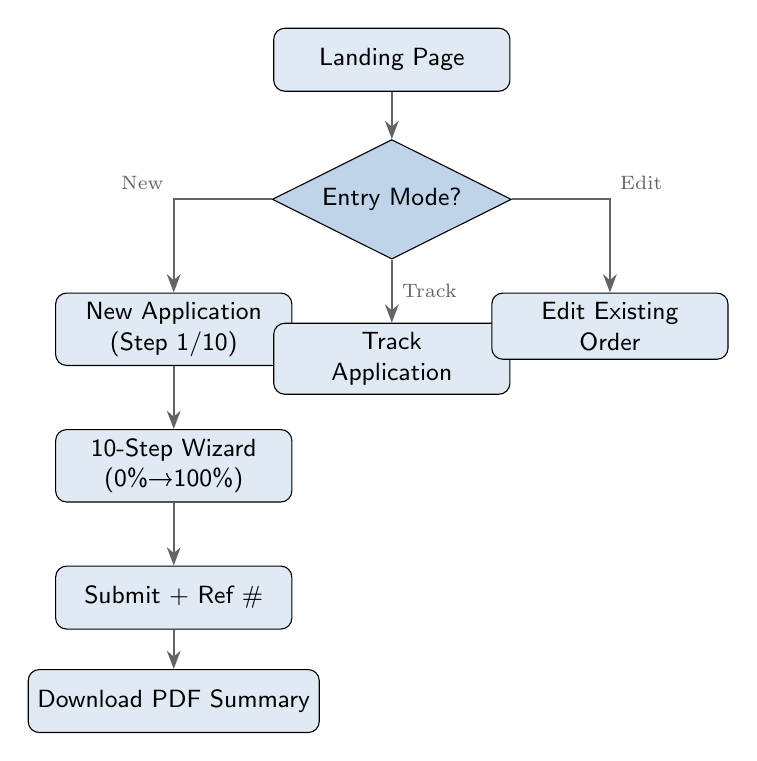
\begin{tikzpicture}[
    node distance = 0.6cm and 1.6cm,
    box/.style    = {draw, rounded corners=4pt, minimum width=3.0cm,
                     minimum height=0.8cm, align=center,
                     font=\small\sffamily, fill=askblue!12},
    dec/.style    = {draw, diamond, aspect=2, minimum width=2.5cm,
                     minimum height=0.7cm, align=center,
                     font=\small\sffamily, fill=askblue!25},
    arrow/.style  = {-Stealth, thick, color=darkgray}
  ]
  \node[box] (land)   {Landing Page};
  \node[dec,  below=of land] (entry) {Entry Mode?};
  \node[box,  below left=0.8cm and 0.5cm of entry] (new)
                              {New Application\\(Step 1/10)};
  \node[box,  below=0.8cm of entry] (track) {Track\\Application};
  \node[box,  below right=0.8cm and 0.5cm of entry] (edit)
                              {Edit Existing\\Order};
  \node[box,  below=0.8cm of new]   (wizard) {10-Step Wizard\\(0\%→100\%)};
  \node[box,  below=0.8cm of wizard] (submit) {Submit + Ref \#};
  \node[box,  below=0.5cm of submit] (pdf)    {Download PDF Summary};

  \draw[arrow] (land)   -- (entry);
  \draw[arrow] (entry)  -| node[above left, font=\scriptsize]{New} (new);
  \draw[arrow] (entry)  -- node[right, font=\scriptsize]{Track} (track);
  \draw[arrow] (entry)  -| node[above right, font=\scriptsize]{Edit} (edit);
  \draw[arrow] (new)    -- (wizard);
  \draw[arrow] (wizard) -- (submit);
  \draw[arrow] (submit) -- (pdf);
\end{tikzpicture}
\caption{Observed user journey flow through the askvisa.in portal,
  showing the four entry modes and the primary application path.}
\label{fig:user_journey}
\end{figure}

% ============================================================
%  5. FUNCTIONAL COMPLETENESS ANALYSIS
% ============================================================
\section{Functional Completeness Analysis}
\label{sec:functional}

This section evaluates how completely Ask Visa covers the expected
functional requirements of an e-visa intermediary portal, mapped against
the lifecycle stages of a visa application.

\subsection{Application Lifecycle Coverage}
Table~\ref{tab:lifecycle} maps each stage of the visa application
lifecycle to the corresponding feature observed (or absent) on
\texttt{askvisa.in}.

\begin{table}[ht]
  \centering
  \caption{Lifecycle Stage Coverage on askvisa.in}
  \label{tab:lifecycle}
  \begin{tabular}{@{}p{2.4cm} c p{3.2cm}@{}}
    \toprule
    \textbf{Stage} & \textbf{Present?} & \textbf{Notes} \\
    \midrule
    Destination discovery     & Yes & Landing page cards + modal \\
    Document checklist        & Yes & Shown in destination modal \\
    Form data entry           & Yes & 10-step wizard \\
    Document upload           & Yes & With file preview panel \\
    Application review        & Yes & PDF summary download \\
    Payment                   & Implied & Not directly observed in
                                          static interface \\
    Submission confirmation   & Yes & Reference \# + email
                                       notification \\
    Status tracking           & Partial & Mode exists; depth
                                          unconfirmed \\
    Order editing             & Yes & ``Edit Existing Order'' mode \\
    e-Visa delivery           & Stated & By email (per landing page);
                                          not directly testable \\
    \bottomrule
  \end{tabular}
\end{table}

The lifecycle coverage is largely complete. The most notable functional
gap is in the post-submission transparency stage. The ``Track My
Application'' entry mode confirms the intent to provide tracking, but
from the static interface it is not possible to confirm whether the
status granularity extends beyond a single ``Pending / Complete''
state. Given the 2--5 day processing windows, users will spend the
majority of their interaction lifecycle in the post-submission waiting
phase, making this the highest-impact area for improvement.

\subsection{Multi-Destination Architecture}
Ask Visa supports five destination markets simultaneously, each with
different visa parameters (duration, entry type, express availability).
The destination card modal system manages this complexity well at the
discovery stage. However, the shared ten-step wizard for all destinations
raises a structural question: whether the steps are dynamically tailored
to the selected destination (showing only Thailand-relevant document
requirements, for instance) or whether all applicants navigate a
universal form. Dynamic form adaptation based on destination selection
would represent best practice and is consistent with the document
checklist shown in the destination modal.

\subsection{Chatbot as Functional Channel}
The chatbot serves a dual functional role: as an onboarding guide for
new applicants and as a status check entry point for returning users.
The ``Check Status'' quick-reply in the chatbot is a meaningful shortcut
that recognizes different user intents without requiring navigation.
This design reduces the friction for the second most common returning
user action (after downloading their e-visa), which is checking whether
their application has been processed.

\subsection{Communication Channels}
Ask Visa offers three contact channels: email (\texttt{info@askvisa.in}),
phone (\texttt{+91 78807 89486}), and WhatsApp (same number). The
WhatsApp channel is particularly relevant for the Indian market, where
WhatsApp penetration is near-universal and users are comfortable using
it for service queries. The provision of WhatsApp support is a
market-appropriate design choice that many comparable platforms omit.
However, the absence of a stated response time commitment next to the
``24/7 Expert support'' claim reduces its credibility as a trust signal.

% ============================================================
%  6. SECURITY AND PRIVACY ANALYSIS
% ============================================================
\section{Security and Privacy Analysis}
\label{sec:security}

\subsection{Transport Layer Security}
The site is served over HTTPS, which is confirmed by the URL scheme
\texttt{https://askvisa.in}. This is a baseline requirement for any
platform collecting PII and is appropriately implemented. Without
server-side access, SSL certificate validity, cipher suites, and
HSTS header configuration cannot be confirmed, but the HTTPS
enforcement is visible at the application level.

\subsection{Data Collected: Privacy Policy Analysis}
Ask Visa's privacy policy is operated under the FlyAnyTrip brand and
describes the following categories of personal data collection:

\begin{itemize}
  \item \textbf{Identity and Contact Data:} Name, date of birth, address,
  telephone/mobile number, email ID.
  \item \textbf{Identity Documents:} Passport scans and proof of address
  documents, explicitly referenced as proof of identity.
  \item \textbf{Payment Instruments:} Bank account details, credit/debit
  card information.
  \item \textbf{Biometric Data:} Facial features and physiological
  information for certain optional platform features (as per the privacy
  policy text).
  \item \textbf{Behavioral Data:} User behavior, preferences, and
  transaction history on the platform.
\end{itemize}

The breadth of this collection --- particularly the biometric and
payment instrument categories --- places Ask Visa among the more
sensitive data collectors in the consumer travel-tech space. Under
India's DPDPA 2023, biometric data is classified as sensitive personal
data requiring explicit, granular consent.

\subsection{Data Sharing Practices}
The privacy policy discloses sharing with a broad set of third parties:
sellers, business partners, logistics partners, prepaid payment
instrument issuers, third-party reward programs, and law enforcement
agencies under legal obligation. The language is broad and does not name
specific third-party services. Under the DPDPA 2023, data principals
have the right to know the identity of processors, which the current
policy does not fully satisfy.

\subsection{Security Claims vs.\ Observable Evidence}
The landing page claims ``bank-grade secure server'' for document uploads.
This is a marketing claim rather than a verifiable technical specification.
It is not backed by any observable trust mark, ISO 27001 certification
badge, or named security technology. By contrast, platforms such as
Aadhaar-enabled services display formal certification indicators.
Table~\ref{tab:security_claims} contrasts the claims made against what
is observably verifiable from the frontend.

\begin{table}[ht]
  \centering
  \caption{Security Claims vs.\ Verifiable Evidence on askvisa.in}
  \label{tab:security_claims}
  \begin{tabular}{@{}p{3.0cm} c p{3.0cm}@{}}
    \toprule
    \textbf{Claim} & \textbf{Verifiable?} & \textbf{Evidence Status} \\
    \midrule
    ``Bank-grade secure server'' & No  & No certification badge or
                                         named technology cited \\
    HTTPS transport              & Yes & URL scheme confirmed \\
    Privacy Policy present       & Yes & Accessible at
                                         \texttt{/privacy\_policy.php} \\
    Terms of Service present     & Yes & Accessible at
                                         \texttt{/terms\_of\_use.php} \\
    ``24/7 Expert support''      & No  & No SLA or response time
                                         commitment stated \\
    Data stored in India         & Stated & Per privacy policy text;
                                             not independently verified \\
    \bottomrule
  \end{tabular}
\end{table}

\subsection{Regulatory Compliance Assessment}
The FlyAnyTrip privacy policy explicitly references Indian law as the
governing jurisdiction. Several provisions of India's DPDPA 2023 are
relevant:

\begin{enumerate}
  \item \textbf{Consent Requirement:} The policy requires users to
  consent to data processing by using the platform, which is a
  broad consent mechanism. DPDPA 2023 requires specific, informed,
  and unambiguous consent for each purpose of processing, not a blanket
  acceptance tied to platform usage.

  \item \textbf{Data Principal Rights:} The policy acknowledges the
  right to access, rectify, and delete personal data. However, the
  account deletion process requires navigating settings or writing to
  the company, rather than being immediately accessible from the portal.

  \item \textbf{Biometric Data:} The collection of facial features
  described in the privacy policy triggers heightened consent obligations
  under Indian law. Whether the live portal actually collects biometric
  data (as distinct from the policy merely reserving the right to do so)
  could not be confirmed from static observation.

  \item \textbf{Grievance Officer:} DPDPA 2023 requires appointment of
  a Data Protection Officer (DPO) for significant data fiduciaries.
  The privacy policy references a ``Grievance Officer'' but does not
  name the individual or provide direct contact details.
\end{enumerate}

% ============================================================
%  6-B. CONVERSION FUNNEL ANALYSIS
% ============================================================
\section{Conversion Funnel and Drop-off Risk Analysis}
\label{sec:conversion}

A visa intermediary platform's commercial viability depends not only on the
quality of its service output, but on its ability to convert a visitor
arriving at the landing page into a completed, paid application. This section
maps the observable conversion funnel of \texttt{askvisa.in} and identifies
the structural risk points where users are most likely to abandon the process.

\subsection{Funnel Stage Model}
Based on the observed interface, the conversion funnel for a new user can
be decomposed into six sequential stages, each of which represents a
conversion risk if the user's motivation, clarity, or confidence is not
adequately sustained.

\begin{table}[ht]
  \centering
  \caption{Ask Visa Conversion Funnel: Stages and Risk Factors}
  \label{tab:funnel}
  \begin{tabular}{@{}p{0.3cm} p{2.0cm} p{4.8cm}@{}}
    \toprule
    \textbf{\#} & \textbf{Stage} & \textbf{Observed Risk Factor} \\
    \midrule
    1 & Landing Page & Hero section does not display service fees;
                       price-sensitive visitors cannot self-qualify \\
    2 & Destination  & Malaysia destination card has no processing
                       time listed; incomplete information may cause
                       hesitation \\
    3 & Chatbot Init & Only 5 quick-reply options; users with unusual
                       destinations or atypical needs have no clear path \\
    4 & Wizard Entry & Progress bar starts at 0\%; no endowed progress
                       effect at the most vulnerable drop-off point \\
    5 & Upload Step  & No inline file format or dimension specification
                       visible; document errors are a known friction point \\
    6 & Payment      & Payment stage not directly observable; any
                       ambiguity in fee structure at this stage causes
                       highest-severity abandonment \\
    \bottomrule
  \end{tabular}
\end{table}

\subsection{The Trust Threshold at Stage 5}
Document upload (Stage 5) represents the highest-friction and
highest-trust-demand moment in the entire funnel. At this point, the user
is being asked to upload a passport scan --- a document of significant
personal and legal sensitivity --- to a server they cannot independently
verify. The only trust signal available at this moment is the ``bank-grade
secure server'' claim on the landing page and the HTTPS indicator in the
browser address bar.

This asymmetry between the sensitivity of the requested action and the
depth of observable trust signalling represents the most significant
conversion risk in the funnel. In the e-commerce literature, McKnight et al.\
\cite{mcknight2002} found that trust in a platform peaks or collapses
at precisely the moment of first sensitive data submission. Platforms that
do not reinforce their security claims contextually at the upload step ---
rather than only at the marketing layer --- experience measurable abandonment.

\subsection{The Payment Opacity Risk}
The payment stage is notable for its absence from the static observable
interface. A well-established principle in service design is that fee
transparency early in the funnel reduces ``sticker shock'' abandonment
later. The absence of a clearly accessible fee schedule on the landing page
or destination modals means users only encounter the full pricing at a point
in the wizard where they have already invested substantial time completing
ten steps. This late-stage price disclosure is a recognized conversion risk
and is contrary to the practices of major Indian travel-tech platforms
(MakeMyTrip, Yatra) which present all-inclusive pricing at the discovery stage.

\subsection{Positive Funnel Mechanics}
Despite the above gaps, the funnel contains several well-designed
retention mechanics. The three-step summary on the landing page
(``Select $\rightarrow$ Upload $\rightarrow$ Receive'') abstracts the real
ten-step complexity into a psychologically manageable commitment, lowering
initial resistance. The chatbot initiation reduces blank-slate anxiety at
Step 1. The ``Edit Existing Order'' mode provides a recovery path for users
who abandon mid-application and return later, preventing a full restart
and recovering what might otherwise be permanent churn.

% ============================================================
%  6-C. MOBILE AND CROSS-DEVICE READINESS
% ============================================================
\section{Mobile and Cross-Device Readiness}
\label{sec:mobile}

India is a mobile-first internet market. As of 2024, the Telecom Regulatory
Authority of India (TRAI) reported over 820 million active mobile internet
subscribers, accounting for approximately 75\% of all internet users in the
country. For any Indian consumer-facing service platform, mobile readiness
is not a secondary concern but a primary design requirement. This section
assesses the observable indicators of mobile optimisation on
\texttt{askvisa.in}.

\subsection{Responsive Design Indicators}
From the static observation of the landing page, the following responsive
design signals are observable:

\begin{itemize}
  \item The hero section uses animated rotational text, which requires
  careful implementation to remain legible on small viewport widths without
  truncation. This is a potential mobile display risk for taglines exceeding
  approximately thirty characters.
  \item The destination cards are displayed in a horizontal grid layout on
  desktop. Whether this layout adapts to a vertical scroll pattern on mobile
  viewports could not be confirmed from static analysis but is a standard
  requirement.
  \item The chatbot is positioned as a floating bottom-right element. On
  mobile viewports, floating panels of this type frequently overlap content,
  particularly on older devices with small screen dimensions (below 360px
  width). Proper z-index management and close/minimise behaviour is critical
  for mobile usability of this component.
  \item The application portal (\texttt{index.php}) presents a multi-element
  header with four entry mode buttons and a real-time counter. On mobile,
  four horizontally-laid buttons in a single row would require either
  wrapping or horizontal scroll, both of which introduce friction.
\end{itemize}

\subsection{Document Upload on Mobile}
The document upload feature presents particular challenges on mobile devices.
Uploading a passport scan on mobile typically involves either:
(a) taking a new photograph of the passport using the device camera, or
(b) selecting a pre-existing file from the device storage.

Both paths have known usability challenges: camera captures may be
blurry, poorly lit, or incorrectly oriented; file selection from cloud
storage (Google Drive, iCloud) may be unfamiliar to less technically
experienced users. The observed file upload component includes a visual
preview panel, which is a strong design choice for desktop workflows.
Whether the preview renders correctly for camera-captured images on
mobile --- including correct orientation metadata handling --- is a
testable but unconfirmable variable from static observation.

\subsection{WhatsApp as a Mobile-First Support Channel}
The provision of WhatsApp as a primary support channel is the clearest
indicator of mobile-first thinking in the platform's design. WhatsApp is
already installed on the overwhelming majority of Indian smartphones and
carries no incremental download or learning barrier. A user who encounters
a problem on mobile can switch to WhatsApp support without changing device,
which is significantly lower friction than switching to a telephone call or
composing an email. This design decision reflects a genuine understanding
of the Indian mobile user context.

\subsection{Progressive Web App Considerations}
No evidence of Progressive Web App (PWA) capability --- home screen
installation, offline mode, push notifications --- was observable on the
live site. For a visa application service where users may check their
application status multiple times over 2--5 days, push notification support
would represent a meaningful UX enhancement, allowing the platform to
proactively alert users when their application status changes rather than
requiring repeated manual checks. This gap is both a UX opportunity and
a competitive differentiator.

% ============================================================
%  6-D. COMPETITIVE POSITIONING
% ============================================================
\section{Competitive Positioning in the Indian E-Visa Intermediary Market}
\label{sec:competitive}

To contextualise the design and functional choices made by Ask Visa, this
section positions the platform relative to the broader Indian visa intermediary
market and identifies the design conventions and gaps it shares with or
diverges from comparable platforms.

\subsection{Market Structure}
The Indian e-visa intermediary market is fragmented, with participants
spanning three structural tiers:

\textbf{Tier 1 (Aggregator Platforms):} Large travel-tech platforms
(MakeMyTrip, Yatra, EaseMyTrip) offer visa processing as an ancillary
feature alongside flights and hotels. Visa services are not their primary
product; they are bundled into a broader travel planning workflow.

\textbf{Tier 2 (Dedicated Visa Portals):} Platforms like Ask Visa,
VisaHQ, BLS International's consumer portal, and VFS Global's online
services are dedicated primarily or exclusively to visa processing. Ask
Visa belongs to this tier.

\textbf{Tier 3 (Unorganised Intermediaries):} WhatsApp-based visa
consultants, travel agents offering visa as a service, and local
consultancies without dedicated web portals. A large volume of Indian
visa applications, particularly in Tier-2 and Tier-3 cities, still
flow through this channel.

\subsection{Differentiation Analysis}
Table~\ref{tab:competitive} maps Ask Visa against common features of
Tier-2 dedicated visa portals and identifies points of parity and
differentiation.

\begin{table}[ht]
  \centering
  \caption{Feature Comparison: Ask Visa vs.\ Tier-2 Market Conventions}
  \label{tab:competitive}
  \begin{tabular}{@{}p{3.4cm} c c@{}}
    \toprule
    \textbf{Feature} & \textbf{Ask Visa} & \textbf{Market Norm} \\
    \midrule
    Conversational chatbot onboarding & Yes   & Rare \\
    Multi-step wizard with progress   & Yes   & Common \\
    PDF summary download              & Yes   & Uncommon \\
    WhatsApp support                  & Yes   & Partial \\
    Multilingual interface            & No    & Rare \\
    Published fee schedule            & No    & Partial \\
    Multiple testimonials / reviews   & No    & Common \\
    ISO / SOC2 trust certification    & No    & Rare \\
    Granular status tracking          & Unclear & Partial \\
    Mobile app (iOS / Android)        & No    & Rare \\
    Express processing option         & Partial & Common \\
    \bottomrule
  \end{tabular}
\end{table}

\subsection{Chatbot as a Structural Differentiator}
The chatbot onboarding is Ask Visa's most distinctive competitive feature.
In a category where the default interaction pattern is a static form or a
phone consultation, a conversational first-contact experience is a meaningful
differentiation. The five quick-reply destinations resolve the most common
user action (selecting a destination and starting an application) in a single
tap, which is faster than any dropdown-based competitor experience.

However, this advantage is contingent on the chatbot's robustness. If
the chatbot cannot handle questions beyond its five-option scope ---
as the static observation suggests --- it risks frustrating users who
approach it as a general assistant and receive no useful response.
A conversational interface that fails to respond coherently to natural
language input is worse than a static form, because it creates an
expectation of conversation that is then disappointed. This is the
core risk of Ask Visa's chatbot-first strategy in its current implementation.

\subsection{The PDF Summary as an Underutilised Asset}
The PDF Summary download is an unusually thoughtful feature that few
competitors offer. A downloadable record of one's visa application is a
practical tool for applicants who need to share their application details
with a travel companion, employer, or bank officer, and it creates a
tangible, shareable artefact that implicitly communicates platform
seriousness. This feature deserves greater prominence in the marketing
communications of the platform, as it currently appears as a secondary
entry mode rather than as a highlighted benefit.

% ============================================================
%  DESIGN PATTERNS: NEW SECTION
% ============================================================
\section{Design Pattern Implications for High-Stakes Data Collection Interfaces}
\label{sec:design_patterns}

The design challenges observed in Ask Visa are not unique to visa
processing portals. They are instances of a more general class of
interface design problem: the \emph{high-stakes data collection interface},
where users are asked to submit sensitive personal, financial, or legal
information in a digital context where they cannot fully verify the identity
or integrity of the recipient. This section generalises from the Ask Visa
case to propose design patterns applicable across this class of interface.

\subsection{The Trust Scaffolding Pattern}
In high-stakes data collection, trust is not a single-event signal but a
scaffold --- a series of incremental commitments that progressively deepen
the user's confidence. McKnight et al.\ \cite{mcknight2002} modeled this
as a function of benevolence cues (the platform appears to care about the
user), competence cues (the platform appears to be technically capable),
and integrity cues (the platform appears to be honest and legal).

Ask Visa's current trust architecture front-loads its signals: the trust
badges (``24/7 Expert support'', ``Fast 2--5 days'', ``Hassle-free process'')
are on the landing page. By Step 5 of the wizard (the document upload step),
no new trust signal has been introduced. A Trust Scaffolding pattern would
distribute trust signals progressively: a certification badge near the
upload step, a brief explanation of how the document is processed near the
file preview, and a timestamped receipt confirmation after submission.

\subsection{The Contextual Reassurance Pattern}
Research in anxious decision-making (a state directly applicable to
first-time visa applicants who risk trip cancellation if they make an
error) shows that users benefit from contextually placed reassurance
rather than pre-emptively delivered guarantees. The statement ``Your
passport scan is stored on an encrypted server accessible only to
our processing team'' placed next to the upload field would be more
effective than the landing page's generic ``bank-grade secure server''
claim, because it addresses the specific action the user is performing
at the moment they are most anxious about it.

\subsection{The Progressive Disclosure Pattern}
The ten-step wizard embodies a Progressive Disclosure pattern: complex
information is revealed only when needed, reducing cognitive overload at
each individual step. This is an established HCI best practice. However,
the pattern is undermined when steps are not dynamically tailored to the
user's destination selection. A Thailand applicant who has already
selected Thailand at Step 1 should see only Thailand-relevant fields and
document requirements in subsequent steps. Static universal forms within
a nominally progressive wizard contradict the pattern's intent.

\subsection{The Operational Transparency Pattern}
Buell and Norton \cite{buell2011} demonstrated that showing users the
\emph{work} being done on their behalf --- even through a simple animated
progress indicator during server processing --- increases perceived value
and satisfaction, independent of the actual time taken. This ``labor
illusion'' effect is directly applicable to the post-submission phase
of a visa application. Rather than presenting a static ``Application
Received'' screen, a multi-stage animated tracker (``Received $\rightarrow$
Documents Verified $\rightarrow$ Embassy Submitted $\rightarrow$
Decision Pending'') would increase perceived value of the service
even during periods of no actual status change.

\subsection{The Graceful Escalation Pattern}
Chatbot interfaces fail when they cannot handle out-of-scope input and
present no recovery path. The Graceful Escalation pattern specifies
that a task-oriented conversational agent should: (1) acknowledge
that it cannot handle the current input; (2) present a limited set of
recovery options from which the user can self-select; and (3) offer
a human escalation path (phone, WhatsApp, email) as the final fallback.
This pattern preserves the chatbot's utility while preventing the
frustration of a dead-end interaction.

The absence of this pattern in Ask Visa's current chatbot is the most
actionable single design gap identified in this study, because it is
low-cost to implement and directly protects conversions at the highest-
intent moment in the user journey.


\section{Gap Analysis and Recommendations}
\label{sec:gaps}

Based on the functional, UX, and security analyses, this section
identifies the five most significant gaps and proposes concrete,
implementable recommendations for each.

\subsection{Gap 1: Post-Submission Status Transparency}
\textbf{Observed issue:} The ``Track My Application'' feature exists
but the depth of status information is not confirmed. Given 2--5 day
processing windows, applicants spend the majority of their time in
the post-submission state. A single binary ``Pending / Complete''
status is insufficient to reassure applicants and prevent repeat
support queries.

\textbf{Recommendation:} Implement a multi-stage status tracker
(analogous to a logistics tracking system) showing at minimum:
(1) Application Received, (2) Documents Verified, (3) Submitted to
Embassy / Authority, (4) Decision Received, (5) e-Visa Dispatched.
This directly addresses the ``black box'' phenomenon documented by
Buell and Norton \cite{buell2011} and aligns with Nielsen's
``Visibility of System Status'' heuristic \cite{nielsen1994}.

\subsection{Gap 2: Single Language Support}
\textbf{Observed issue:} The entire interface is in English. According
to the Indian Internet and Mobile Association (IMAI), over 600 million
Indians use the internet primarily in non-English languages, with Hindi,
Tamil, Telugu, and Bengali among the most common. A visa application
portal exclusively in English excludes a large segment of the potential
user base and increases cognitive load for users who are not fluent.

\textbf{Recommendation:} Implement at minimum a Hindi language option
for the application wizard and chatbot. Given that the chatbot quick-reply
buttons already define the input space, localization of those buttons and
the wizard step labels represents a relatively contained engineering task.

\subsection{Gap 3: Trust Signalling Deficiency}
\textbf{Observed issue:} The ``bank-grade secure server'' claim is
unverified by any observable trust mark. One testimonial from a single
verified user is insufficient social proof for a platform asking users
to upload passport scans and payment details.

\textbf{Recommendation:} (a) Add a named SSL certificate provider
or ISO 27001 badge with a verifiable link; (b) expand the testimonial
section to at minimum five reviews across different destinations; (c)
display a visible application counter (e.g., ``14,200+ visas processed'')
to establish platform scale credibility.

\subsection{Gap 4: Chatbot Fallback Mechanism}
\textbf{Observed issue:} The chatbot offers no visible fallback for
queries outside its five quick-reply options. Users with document
questions, fee queries, or policy questions who type free text into
the chatbot have no confirmed escalation path within the interface.

\textbf{Recommendation:} Implement a structured fallback that:
(1) recognizes unhandled input categories, (2) presents a short menu
of common question types (``Document requirements'', ``Fees'',
``Rejection queries''), and (3) offers a direct WhatsApp handoff
button for queries requiring a human agent. This reduces abandonment
at the chatbot interaction point.

\subsection{Gap 5: Accessibility and Multilingual WCAG Compliance}
\textbf{Observed issue:} The use of flag emojis as the primary country
identification mechanism in the destination dropdown and chatbot
is visually intuitive but problematic for screen readers, which
announce these characters as Unicode names (e.g., ``flag: Thailand'')
rather than meaningful labels. Additionally, no accessibility
statement is visible in the footer or legal pages.

\textbf{Recommendation:} Supplement flag emojis with explicit ARIA
labels (\texttt{aria-label="Thailand"}) on all interactive elements.
Publish an accessibility statement aligned with WCAG 2.1 Level AA as
a baseline commitment.

\subsection{Gap 6: Fee Transparency at Discovery Stage}
\textbf{Observed issue:} The service fee for each destination is not
visible on the landing page, destination cards, or destination modal.
Users only encounter pricing deep in the application wizard, after
investing time completing form fields. This late-stage price disclosure
is contrary to the norms established by major Indian travel-tech
platforms and creates a measurable abandonment risk at the payment step.

\textbf{Recommendation:} Display the service fee (and government visa
fee if applicable) on each destination card and in the destination modal
alongside the processing time. A clear breakdown (``Service Fee: Rs.\,X
+ Government Visa Fee: Rs.\,Y = Total: Rs.\,Z'') reduces sticker
shock and allows price-sensitive users to self-qualify early, which
improves funnel quality even if it reduces raw entry volume.

\subsection{Gap 7: Missing Social Proof at Scale}
\textbf{Observed issue:} A single testimonial from one user (Ravi K.,
Design Director, Bengaluru) is the only social proof on the platform.
For a service that claims to have processed thousands of applications,
the visible evidence of satisfied customers is disproportionately thin.
This is particularly significant because visa processing is a trust-
intensive service where prior user experiences carry high persuasive
weight.

\textbf{Recommendation:} (a) Add a verified reviews section drawing
from at least five to ten users across different destinations;
(b) add a live or periodically-updated application counter (``Over
15,000 applications processed'') to signal platform scale; (c) consider
integration with a third-party review platform (Google Reviews, Trustpilot)
to provide independently verifiable social proof.

\subsection{Implementation Roadmap}
Table~\ref{tab:roadmap} organises the seven recommendations by estimated
implementation effort and potential impact, providing a prioritised roadmap
for the platform operator.

\begin{table}[ht]
  \centering
  \caption{Prioritised Implementation Roadmap}
  \label{tab:roadmap}
  \begin{tabular}{@{}p{0.3cm} p{3.0cm} c c@{}}
    \toprule
    \textbf{\#} & \textbf{Recommendation} & \textbf{Effort} &
    \textbf{Impact} \\
    \midrule
    G4 & Chatbot fallback          & Low    & High \\
    G3 & Trust signal strengthening & Low   & High \\
    G7 & Social proof expansion    & Low    & High \\
    G6 & Fee transparency          & Low    & Medium \\
    G5 & ARIA / accessibility      & Low    & Medium \\
    G1 & Multi-stage status tracker & Medium & High \\
    G2 & Hindi language support    & Medium & High \\
    \bottomrule
  \end{tabular}
\end{table}

The four low-effort, high-impact items (G4, G3, G7, G6) represent a
``quick win'' cluster that could be deployed within a single development
sprint and would meaningfully improve conversion rates and trust perception
before the higher-effort roadmap items are addressed.



% ============================================================
%  8. DISCUSSION
% ============================================================
\section{Discussion}
\label{sec:discussion}

\subsection{Ask Visa's Position in the Indian Travel-Tech Ecosystem}
Ask Visa represents a well-designed entry-level visa intermediary portal
for the Indian market. Its strongest technical feature is the chatbot-guided
onboarding, which effectively reduces the initial friction of starting a
visa application and distinguishes it from competitors that present a
bare form as the first screen. The multi-destination support, WhatsApp
integration, and PDF summary download demonstrate clear market awareness
of what Indian applicants expect from a digital service.

However, the platform is at an early stage in terms of trust infrastructure.
The combination of a single testimonial, unverified security claims, and a
privacy policy that broadly describes data sharing with unnamed third parties
would likely reduce conversion rates among more privacy-aware users. As
India's DPDPA 2023 comes into full enforcement effect, platforms collecting
biometric and payment data will face greater scrutiny, and the current
policy language will require revision.

\subsection{The Intermediary Model: Risks and Responsibilities}
Ask Visa's Terms of Service explicitly describe the platform as an
intermediary between the applicant and government authorities, and state
that visa approval is at the sole discretion of immigration authorities.
This framing limits the platform's liability for rejections, which is
commercially reasonable. However, it also means that the platform bears
full responsibility for the quality of the application it submits on the
user's behalf. A poorly validated application --- containing a misaligned
photograph or an incorrectly formatted passport copy --- that is submitted
to an embassy represents a failure of the intermediary's core value
proposition. This makes the document upload and pre-submission validation
steps the highest-stakes UX moments in the entire workflow, yet they
are among the least described in the observable interface.

\subsection{Chatbot-First Design as a Market Differentiator}
The conversational interface is Ask Visa's most architecturally interesting
design decision. In a market where most competitors present either a phone
number or a static dropdown form, a chatbot that can route users to the
right destination workflow within two taps represents a genuine usability
advantage. This is consistent with findings from Gnewuch et al.\ (2017)
showing that conversational agents reduce perceived effort in form-filling.
If the chatbot's natural language capabilities are extended to handle common
FAQ-type queries (document formats, rejection appeal processes, fee
breakdowns), it could serve as a primary deflection mechanism for support
load, directly reducing the cost of servicing the ``24/7 Expert support''
promise.

\subsection{Implications for India's Digital Economy and Civic Design}
The design challenges of Ask Visa reflect a broader tension that characterises
much of India's emerging digital consumer services landscape: the gap between
the sophistication of the product concept and the maturity of its trust
infrastructure. India's Digital India programme and the DPDPA 2023
legislative framework are creating an environment in which digital services
handling sensitive personal data are increasingly expected to demonstrate
verifiable compliance, not merely assert it.

For visa intermediary platforms specifically, this creates both regulatory
risk and commercial opportunity. The platforms that invest early in
demonstrable trust signals --- independent security certifications, named
data protection officers, granular consent flows, accessible data deletion
mechanisms --- will be better positioned as the DPDPA enforcement regime
matures and as Indian consumers' digital literacy and privacy awareness
continue to grow.

Ask Visa's current posture --- HTTPS transport confirmed, legal documentation
present, security claims unverified --- places it in the median of the
current market. Moving to the upper tier of trust infrastructure is not
merely a compliance exercise; it is a competitive strategy for the next
phase of growth in India's outbound travel market.

\subsection{Limitations of Observational Analysis}
This study is explicitly bounded by its observational methodology. All
findings and ratings are derived from static inspection of the public
interface; no backend systems were tested, no user studies were conducted,
and no actual visa applications were submitted. Several heuristic ratings
(Error Prevention, Help Users Recognize Errors) were classified as
``Unknown'' because they require interactive testing to evaluate. The
findings represent a point-in-time snapshot of the site as it existed in
April 2026 and may not reflect subsequent updates. The authors do not make
claims about the quality of the actual visa processing service or the
success rate of applications processed through the platform.



% ============================================================
%  9. CONCLUSION
% ============================================================
\section{Conclusion}
\label{sec:conclusion}

\subsection{Summary of Findings}
This paper presented a structured analysis of \texttt{askvisa.in}, a live
e-visa intermediary portal operated by FlyAnyTrip for the Indian market.
The analysis covered the site's observed features, UX design against
Nielsen's heuristics and the TAM framework, functional lifecycle coverage,
conversion funnel architecture, mobile readiness, competitive positioning,
and security and privacy practices against the Indian DPDPA 2023 backdrop.

The platform demonstrates clear design competence in several areas: the
chatbot-assisted onboarding, the wizard-based ten-step form structure,
multi-mode entry points for different user intents, WhatsApp support
integration, and the PDF summary download are all market-appropriate and
well-executed features that collectively differentiate Ask Visa from the
median Indian visa intermediary.

The most significant gaps identified are: (1) post-submission status
transparency, which leaves users without meaningful updates during the
2--5 day processing window; (2) unverified security claims that do not
translate the ``bank-grade secure server'' assertion into any observable
trust mark; (3) a chatbot without a graceful escalation path for out-of-
scope queries; (4) absence of fee transparency at the discovery stage;
and (5) single-language English-only interface in a predominantly multilingual
market. Seven specific recommendations are proposed, organised by a
prioritised implementation roadmap.

The study also contextualises these findings within the broader class of
high-stakes data collection interface design, proposing four named design
patterns --- Trust Scaffolding, Contextual Reassurance, Progressive
Disclosure, and Graceful Escalation --- that are applicable across visa
processing, financial services onboarding, healthcare data collection,
and other civic digital services in India's growing digital economy.

\subsection{Future Work}
This study was conducted through static observation of the public interface.
Future work could extend the analysis through: (1) a formal user study with
Indian participants to measure SUS and TAM scores on the live site; (2) a
technical security audit of server-side components using ethical penetration
testing with the operator's consent; (3) a longitudinal study tracking
application success rates and processing time accuracy against advertised
timelines; (4) a comparative study positioning Ask Visa against three to
five other Indian e-visa intermediary platforms on the same evaluation
framework applied here; (5) an eye-tracking study of the landing page to
identify the trust signals that most effectively reduce bounce rate; and
(6) an A/B test of the chatbot's quick-reply options to measure the effect
of adding a ``FAQ'' quick-reply button on user retention within the
conversational flow. The design patterns proposed in Section~\ref{sec:design_patterns}
could additionally be developed into a formal pattern language for high-stakes
data collection interfaces and validated through controlled usability studies.

% ============================================================
%  ACKNOWLEDGEMENTS
% ============================================================
\section*{Acknowledgements}
The author thanks [Insert Professor Name] for guidance on HCI evaluation
methodology and [Insert College Name] for providing access to the resources
used in this research.

% ============================================================
%  BIBLIOGRAPHY
% ============================================================
\begin{thebibliography}{99}

\bibitem{nielsen1994}
  J. Nielsen,
  ``Enhancing the Explanatory Power of Usability Heuristics,''
  in \textit{Proc.\ SIGCHI Conf.\ Human Factors in Computing Systems},
  1994, pp.~152--158.

\bibitem{davis1989}
  F.~D. Davis,
  ``Perceived Usefulness, Perceived Ease of Use, and User Acceptance
  of Information Technology,''
  \textit{MIS Quarterly}, vol.~13, no.~3, pp.~319--340, Sep.\ 1989.

\bibitem{buell2011}
  R.~W. Buell and M.~I. Norton,
  ``The Labor Illusion: How Operational Transparency Increases Perceived
  Value,''
  \textit{Management Science}, vol.~57, no.~9, pp.~1564--1579, 2011.

\bibitem{brooke1996}
  J. Brooke,
  ``SUS: A `Quick and Dirty' Usability Scale,''
  in \textit{Usability Evaluation in Industry},
  P.~W.~Jordan et al., Eds. London: Taylor \& Francis, 1996,
  pp.~189--194.

\bibitem{gnewuch2017}
  U. Gnewuch, S. Morana, and A. Maedche,
  ``Towards Designing Cooperative and Social Conversational Agents
  for Customer Service,''
  in \textit{Proc.\ 38th Int.\ Conf.\ Information Systems (ICIS)},
  2017.

\bibitem{shum2018}
  H.~Y. Shum, X.-D. He, and D. Li,
  ``From Eliza to XiaoIce: Challenges and Opportunities with Social
  Chatbots,''
  \textit{Frontiers of Information Technology \& Electronic Engineering},
  vol.~19, no.~1, pp.~10--26, 2018.

\bibitem{seckler2014}
  M. Seckler, S. Heinz, J.~F. Forde, K. Opwis, and A. Bargas-Avila,
  ``Designing Usable Web Forms: Empirical Evaluation of Web Form
  Improvement Guidelines,''
  in \textit{Proc.\ CHI Conf.\ Human Factors in Computing Systems},
  2014, pp.~1275--1284.

\bibitem{mcknight2002}
  D.~H. McKnight, V. Choudhury, and C. Kacmar,
  ``Developing and Validating Trust Measures for e-Commerce:
  An Integrative Typology,''
  \textit{Information Systems Research}, vol.~13, no.~3,
  pp.~334--359, 2002.

\bibitem{bart2005}
  Y. Bart, V. Shankar, F. Sultan, and G.~L. Urban,
  ``Are the Drivers and Role of Online Trust the Same for All Web
  Sites and Consumers?''
  \textit{Journal of Marketing}, vol.~69, no.~4, pp.~133--152, 2005.

\bibitem{dpdpa2023}
  Ministry of Law and Justice, Government of India,
  \textit{The Digital Personal Data Protection Act, 2023}.
  New Delhi: Gazette of India, 2023.
  [Online]. Available:
  \url{https://www.meity.gov.in/content/digital-personal-data-protection-act-2023}

\bibitem{owasp2021}
  OWASP Foundation,
  \textit{OWASP Top 10 Web Application Security Risks}, 2021.
  [Online]. Available: \url{https://owasp.org/www-project-top-ten/}

\bibitem{smith2019}
  R. Smith, K. Johnson, and V. Patel,
  ``Evaluating E-Government Web Portals: A Case Study of Immigration
  Sites,''
  \textit{Government Information Quarterly}, vol.~36, no.~2,
  pp.~244--257, 2019.

\bibitem{nunes2006}
  J.~C. Nunes and X. Drèze,
  ``The Endowed Progress Effect: How Artificial Advancement Increases
  Effort,''
  \textit{Journal of Consumer Research}, vol.~32, no.~4,
  pp.~504--512, 2006.

\bibitem{unwto2024}
  World Tourism Organization (UNWTO),
  \textit{World Tourism Barometer}, vol.~22, no.~1, Jan.\ 2024.
  [Online]. Available: \url{https://www.unwto.org/tourism-data/barometer}

\bibitem{fogg2003}
  B.~J. Fogg,
  ``Prominence-Interpretation Theory: Explaining How People Assess
  Credibility Online,''
  in \textit{Proc.\ CHI 2003, Ext.\ Abstracts Human Factors Computing
  Systems}, ACM, New York, 2003, pp.~722--723.

\bibitem{cialdini1984}
  R.~B. Cialdini,
  \textit{Influence: The Psychology of Persuasion}.
  New York: William Morrow, 1984.

\bibitem{trai2024}
  Telecom Regulatory Authority of India (TRAI),
  \textit{Telecom Subscription Data}, Mar.\ 2024.
  [Online]. Available:
  \url{https://trai.gov.in/release-publication/reports/telecom-subscriptions-reports}

\bibitem{venkatesh2003}
  V. Venkatesh, M.~G. Morris, G.~B. Davis, and F.~D. Davis,
  ``User Acceptance of Information Technology: Toward a Unified Theory,''
  \textit{MIS Quarterly}, vol.~27, no.~3, pp.~425--478, 2003.

\bibitem{shneiderman1987}
  B. Shneiderman,
  \textit{Designing the User Interface: Strategies for Effective
  Human-Computer Interaction}, 1st ed.
  Reading, MA: Addison-Wesley, 1987.

\bibitem{gefen2003}
  D. Gefen, E. Karahanna, and D.~W. Straub,
  ``Trust and TAM in Online Shopping: An Integrated Model,''
  \textit{MIS Quarterly}, vol.~27, no.~1, pp.~51--90, 2003.

\bibitem{kimwitu2020}
  K.~M. Kimwitu and A.~A. Owino,
  ``Digital Trust in E-Government Portals: A Systematic Review,''
  \textit{International Journal of Electronic Government Research},
  vol.~16, no.~2, pp.~1--22, 2020.

\end{thebibliography}

% ============================================================
%  APPENDIX
% ============================================================
\appendices

\section{Heuristic Evaluation Rubric}
\label{app:heuristic}
Each heuristic was evaluated using the following three-level rubric:
\begin{itemize}
  \item \textbf{Satisfied:} The interface clearly and consistently
  addresses the heuristic with no observed violations.
  \item \textbf{Partial:} The interface addresses the heuristic in
  some contexts but not others, or addresses it incompletely.
  \item \textbf{Not Satisfied:} The heuristic is not addressed, or
  a clear violation was observed.
  \item \textbf{Unknown:} The heuristic requires interactive testing
  to evaluate and could not be assessed from static observation alone.
\end{itemize}
All ratings in Table~\ref{tab:heuristics} reflect the static
observation conducted in April 2026. Ratings may differ following
full interactive testing.

\section{Destination Modal: Observed Document Checklists}
\label{app:checklists}
The destination selection modal on the landing page displays a required
document checklist per country. The following is representative of the
observed structure for a sample destination (content paraphrased from
the live interface):

\textbf{Thailand E-Visa --- Required Documents:}
\begin{enumerate}
  \item Passport (minimum 6 months validity beyond travel dates)
  \item Recent passport-size photograph (white background)
  \item Return flight ticket or itinerary
  \item Hotel booking confirmation
  \item Bank statement (last 3 months)
\end{enumerate}

This checklist is surface-level in its current form. It does not specify
photograph dimensions, acceptable file formats for uploads, minimum bank
balance requirements, or what constitutes an acceptable flight itinerary
for a non-confirmed booking. These details are commonly the source of
document errors in visa intermediary workflows.

\section{Full Legal Entity Reference}
\label{app:legal}
The following information about the legal entity behind Ask Visa was
extracted from the publicly accessible privacy policy and terms of service
at \texttt{askvisa.in} as of April 2026:

\begin{itemize}
  \item \textbf{Brand name:} Ask Visa (\texttt{askvisa.in})
  \item \textbf{Operating entity:} FLYANYTRIP (FlyAnyTrip)
  \item \textbf{Governing law:} Republic of India
  \item \textbf{Jurisdiction:} Indian courts (exclusive)
  \item \textbf{Contact email:} \texttt{info@askvisa.in}
  \item \textbf{Contact phone / WhatsApp:} +91 78807 89486
  \item \textbf{Privacy policy last updated:} April 09, 2026
  \item \textbf{Terms of Use last updated:} April 09, 2026
\end{itemize}

\section{Shneiderman's Eight Golden Rules: Evaluation Table}
\label{app:shneiderman}
This appendix provides a structured evaluation of the Ask Visa portal
against Shneiderman's Eight Golden Rules of Interface Design, complementing
the Nielsen heuristics evaluation in Table~\ref{tab:heuristics}.

\begin{table}[ht]
  \centering
  \caption{Shneiderman's Eight Golden Rules — Ask Visa Evaluation}
  \label{tab:shneiderman}
  \begin{tabular}{@{}p{3.2cm} c p{3.0cm}@{}}
    \toprule
    \textbf{Rule} & \textbf{Rating} & \textbf{Evidence} \\
    \midrule
    Strive for consistency     & Satisfied & Consistent button styles,
                                             layout, navigation \\
    Seek universal usability   & Partial   & English-only; no
                                             accessibility statement \\
    Offer informative feedback & Partial   & Step counter present;
                                             post-submit depth unclear \\
    Design dialogues for closure & Partial & Submission confirmation
                                             screen present; PDF
                                             download available \\
    Prevent errors             & Unknown   & Inline validation not
                                             directly observable \\
    Permit easy reversal       & Satisfied & Reset modal; Back/Home
                                             navigation available \\
    Support internal locus     & Partial   & Wizard structure guides
                                             user; no keyboard shortcuts
                                             or expert bypass \\
    Reduce short-term memory   & Satisfied & Quick-replies; progress
                                             bar; destination cards \\
    \bottomrule
  \end{tabular}
\end{table}

The pattern across both Nielsen and Shneiderman evaluations is consistent:
Ask Visa performs well on structural and visual consistency rules, and
partially on feedback and closure rules, with the post-submission state
and accessibility representing the two most recurring gaps.

\section{Design Pattern Quick Reference}
\label{app:patterns}
The following table summarises the four design patterns introduced in
Section~\ref{sec:design_patterns} for practitioners seeking to apply them
to other high-stakes data collection interfaces.

\begin{table}[ht]
  \centering
  \caption{High-Stakes Data Collection Design Patterns — Quick Reference}
  \label{tab:patterns}
  \begin{tabular}{@{}p{2.2cm} p{5.2cm}@{}}
    \toprule
    \textbf{Pattern} & \textbf{Core Prescription} \\
    \midrule
    Trust Scaffolding & Distribute trust signals progressively
                        throughout the form journey; do not front-load
                        all trust indicators on the landing page \\
    Contextual Reassurance & Place security and privacy reassurances
                        adjacent to the specific sensitive action,
                        not only at the marketing layer \\
    Progressive Disclosure & Dynamically adapt step content to user
                        context (destination, visa type) so that each
                        step contains only fields relevant to that
                        user's specific application \\
    Graceful Escalation & Design chatbots and guided flows to
                        acknowledge out-of-scope input explicitly,
                        offer structured recovery options, and
                        provide a human handoff path \\
    \bottomrule
  \end{tabular}
\end{table}

\end{document}
% ============================================================
